% !TeX encoding = UTF-8

\chapter{IMPLEMENTAÇÃO DAS TÉCNICAS}\label{ch:implementacao}
Este capítulo tem como objetivo apresentar, de forma mais detalhada, todo o processo de implementação realizado no presente trabalho, com o intuito de alcançar os objetivos especificados no Capítulo 1.

\section{REALIZAÇÃO DA COLETA DE DADOS}
Tendo em vista as ferramentas necessárias para realizar à coleta das séries temporais que serão utilizadas para o treinamento e testes da RNA, foi desenvolvido um método de automatização de aquisição dos \textit{DataFrames} das ações que serão coletadas para a análise.

Inicialmente, foi criada uma interface em Python que contém a assinatura do método que as classes das empresas deverão implementar. Após isso, foram criadas as classes para as respectivas empresas, definidas no seção 4.2. Para exemplificar o que está sendo exposto, o Código 3 demonstra, de forma mais intuituva, a implementação do atual procedimento.
\codigoPython\
\lstinputlisting[label=cod:exempla-coleta, caption=Implementação da interface Empresa em Python]{src/empresa.py}

Analisando este código, pode-se observar o desenvolvimento da interface "Empresa"\, e da classe "Apple", que implementa esta interface através do parâmetro (Empresa) em sua definição. Também é possível observar, na classe Apple, a implementação do método construtor "\_\_init\_\_"\, que contém seu respectivo nome e código, necessário para realizar a busca. O método "executa\_busca", por sua vez, faz uma chamada ao objeto que realizará a coleta das respectivas ações, passando seus parâmetros como valor. O Código 4 ilustra a implementação do objeto de busca.

\lstinputlisting[language=Python, label=cod-crawler, caption=Implementação do objeto Crawler que realiza a busca das ações]{src/crawler.py}

O Código 4 utiliza a biblioteca pandas para realizar a coleta das ações. Pode-se observar que o método construtor "\_\_init\_\_"\, recebe o nome e o código da empresa que faz a chamada de sua instância. Também é possível analisar o método "executa\_busca"\, implementado, que realiza a chamada da função "web.DataReader"\,
passando quatro parâmetros, sendo eles:
\begin{enumerate}
\item Código da empresa;
\item API que será realizada a busca;
\item Data de inicial da coleta;
\item Data final da coleta.
\end{enumerate}

Após a realização da requisição, a API retorna um arquivo com as ações entre as respectivas datas, no formato especificado na seção 4.4.2, formando assim, o \textit{DataFrame} inicial das empresas. Este procedimento foi realizado para todas as empresas que são analisadas neste trabalho.

Posteriormente, são analisadas as séries específicas de cada empresa, através de seus valores diários de abertura. O período coletado foi de 09/04/2001 a 31/08/2017.

Iniciando por ordem alfabética, as ações da Amazon contém os valores mais altos dentre as empresas estudadas. No período coletado, seu valor de abertura apresentou um mínimo de 5,91 e um máximo de 1069,55 dólares Americanos (USD), evidenciando seu crescimento e valorização. O Gráfico 2 representa o comportamento desta série.
\begin{grafico}[h]
	\centering
	\centerline{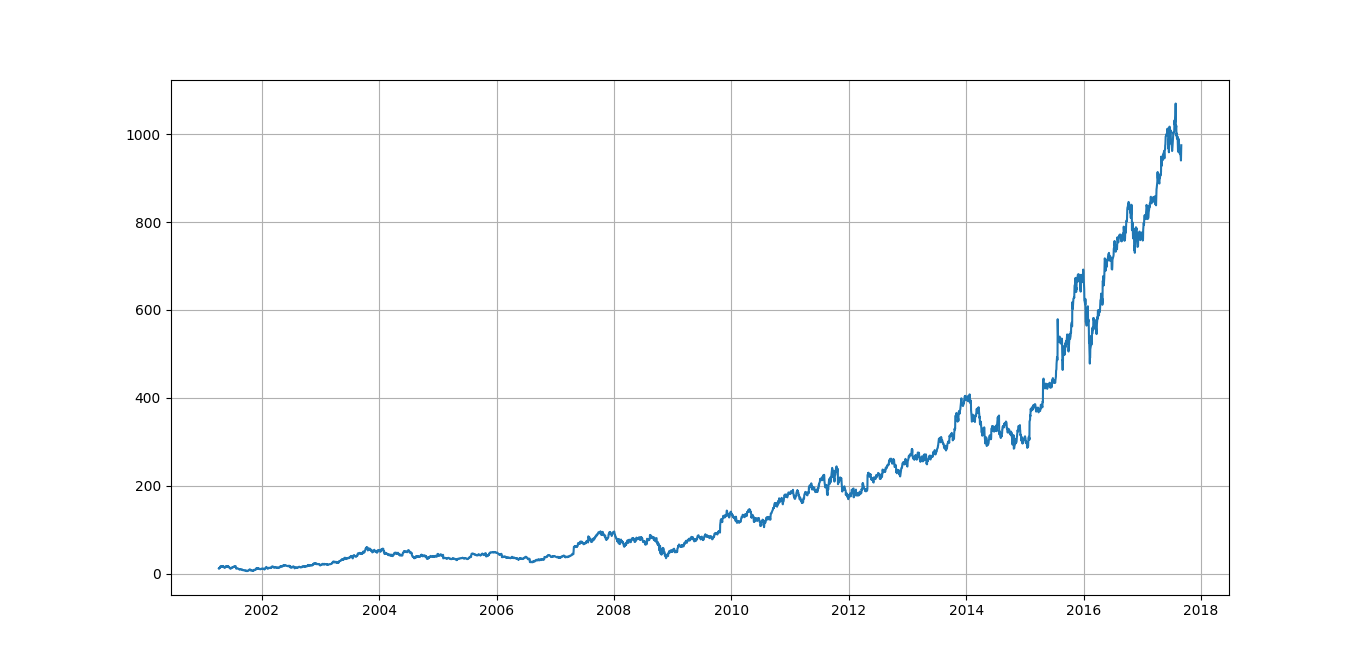
\includegraphics[scale=4]{amazon_coletado}}
	\caption{Valores de abertura das ações da Amazon}
	\fonte{Elaborado pelo autor}
	\label{exec-amazon-coleta}
\end{grafico}

As ações da Apple contam com seus valores mais constantes, sem grande ascenção se comparada a Amazon. Seu valor de abertura apresentou um mínimo de 0,93 e um máximo de 163,80 USD. O Gráfico 3 representa o comportamento desta série.

As ações da Cisco, Intel e Microsoft possuem os valores mais equilibrados dentre as empresas selecionadas. O valor de abertura mínimo apresentado pela Cisco, no período coletado, foi de 8,45 enquanto seu valor máximo foi de 34,46 USD. Já a Intel, apresentou um valor um mínimo de 12,17 e um máximo de 38,25 USD. Por fim, a Microsoft também apresentou uma série bem equilibrada no período coletado, variando entre um valor mínimo de 15,20 e um máximo de 74,34 USD. Os Gráficos 4, 5 e 6 mostram, de forma mais intuitiva, as ações da Cisco, Intel e Microsoft, respectivamente. 	
\begin{grafico}[h]
	\centering
	\centerline{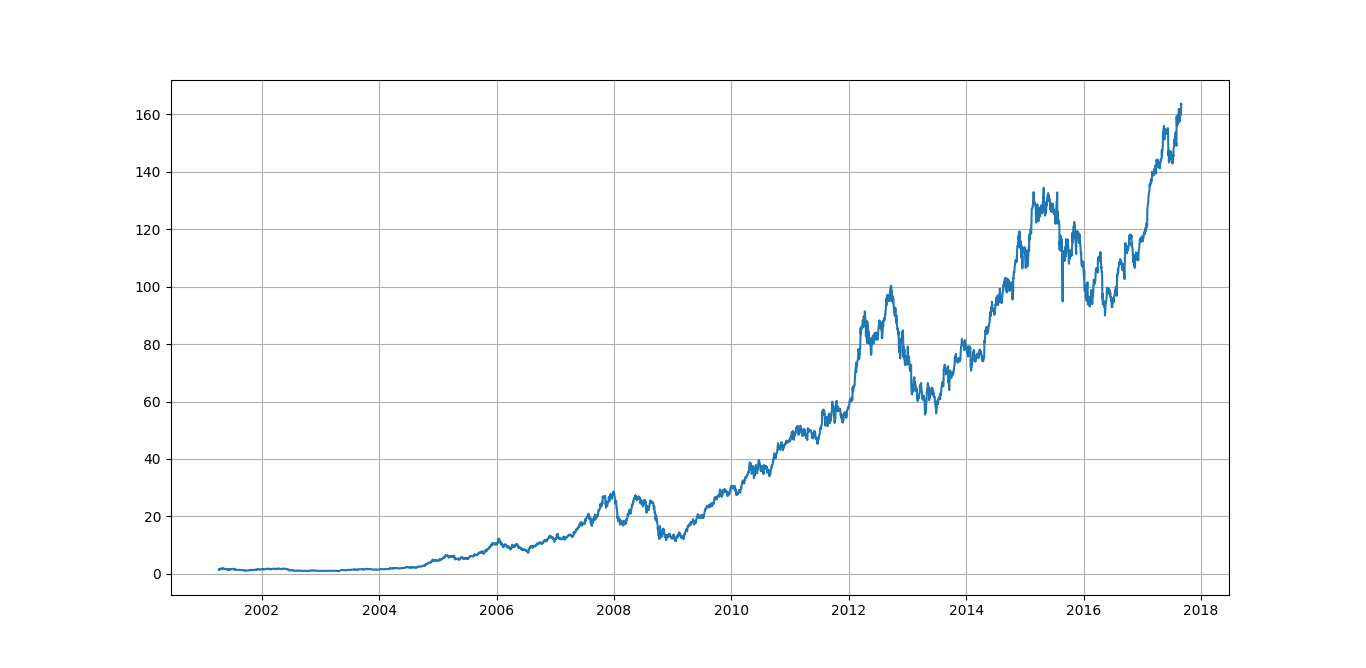
\includegraphics[scale=4]{apple_coletado}}
	\caption{Valores de abertura das ações da Apple}
	\fonte{Elaborado pelo autor}
	\label{exec-apple-coleta}
\end{grafico}

\begin{grafico}[h]
	\centering
	\centerline{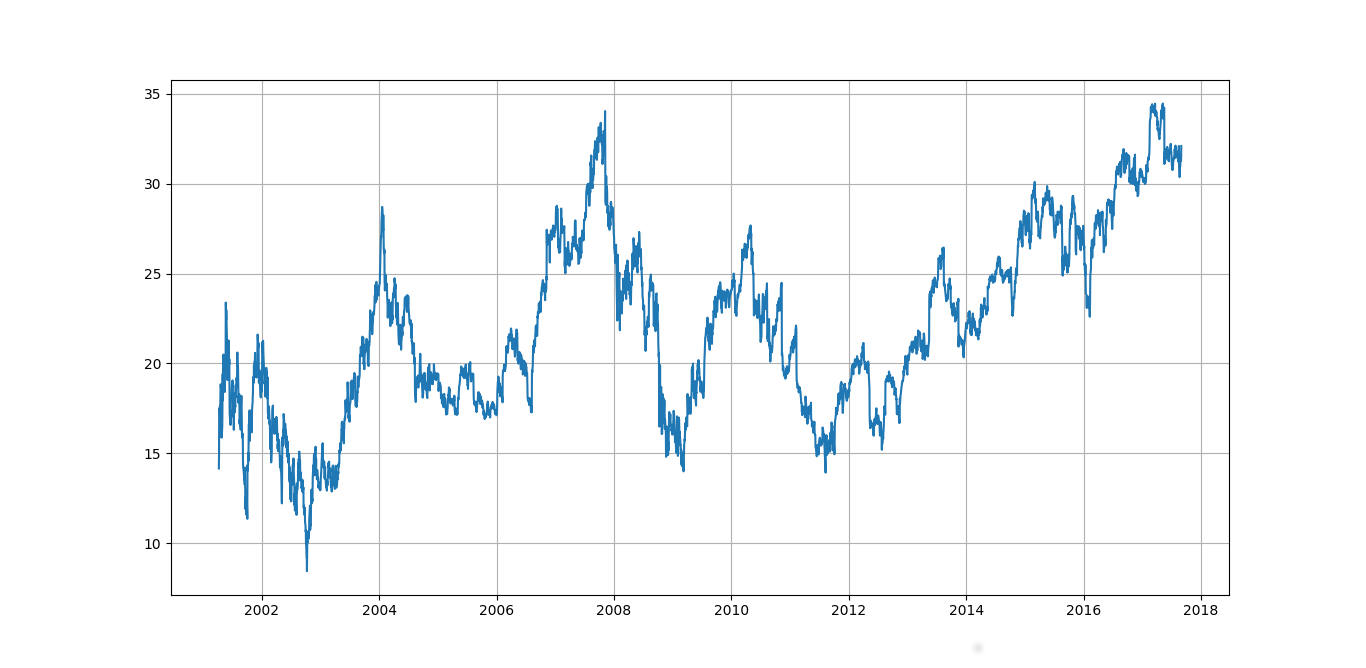
\includegraphics[scale=4]{cisco_coletado}}
	\caption{Valores de abertura das ações da Cisco}
	\fonte{Elaborado pelo autor}
	\label{exec-cisco-coleta}
\end{grafico}
 
\begin{grafico}[h]
	\centering
	\centerline{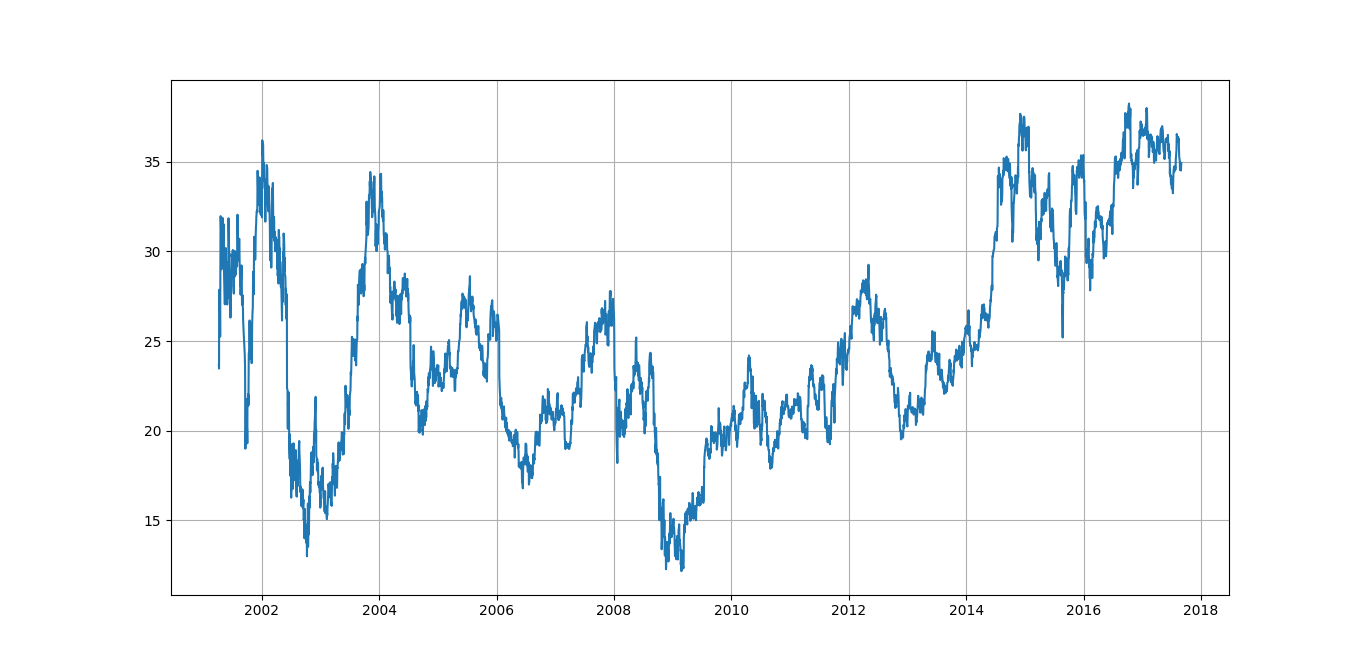
\includegraphics[scale=4]{intel_coletado}}
	\caption{Valores de abertura das ações da Intel}
	\fonte{Elaborado pelo autor}
	\label{exec-intel-coleta}
\end{grafico}

\begin{grafico}[h]
	\centering
	\centerline{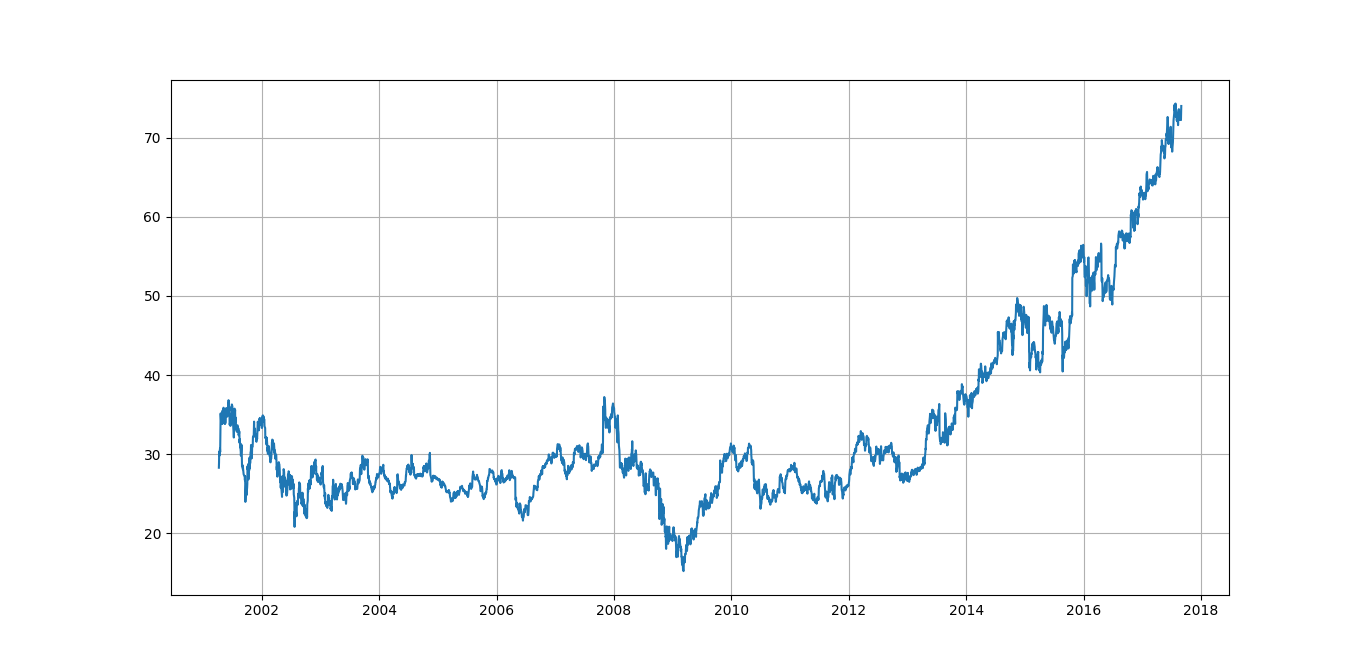
\includegraphics[scale=4]{microsoft_coletado}}
	\caption{Valores de abertura das ações da Microsoft}
	\fonte{Elaborado pelo autor}
	\label{exec-microsoft-coleta}
\end{grafico}

\clearpage
\section{EXPLORANDO O \textit{DATAFRAME}}
O refinamento do modelo de dados coletado é de suma importância para agregar valor às informações do \textit{DataFrame} de cada empresa. Como especificado na Seção 4.3.1, é necessário calcular alguns indicadores técnicos, que são consideradas informações expressivas que influenciam diretamente nos valores das ações.

Para desenvolver o cálculo das médias móveis de 10 e 26 dias, foi formada uma equação levando em consideração o exposto na Seção 4.3.1, o que proporciona de uma forma mais clara como realizar a implementação do algoritmo. A equação (5.1) demonstra este procedimento:
\begin{equation}\label{eq:MMS}
M_t = \dfrac{Z_t + Z_{t-1} + \dots + Z_{t-k+1}}{k},
\end{equation}
onde k é a quantidade de dias que se deseja calcular a média, t é o índice iterador da sequência que está sendo calculada e Z é o valor de fechamento da ação no momento t. A partir disto, foi desenvolvida uma função que realiza este cálculo. O Código 5 ilustra com detalhes esta implementação. 
\lstinputlisting[language=Python, label=cod-media-movel, caption=Implementação da função que realiza o cálculo da média móvel]{src/media-movel.py}

O Código 5 recebe como parâmetro o índice do \textit{DataFrame} e a quantidade de dias que se deseja calcular a média móvel. O algoritmo encontra este índice e, a partir disso, faz um incremento com o valor de fechamento. Após atingir o limite de incrementos necessários, levando em consideração a quantidade de dias, realiza a divisão e salva o valor em uma nova coluna do \textit{DataFrame}.

Já para o cálculo do indicador técnico MACD, o mesmo é realizado de forma mais simples com o auxílio da biblioteca pandas. O Código 6 cria uma nova coluna ao \textit{DataFrame} e realiza o cálculo da diferença, utilizando a função "sub", entre as duas médias móveis.
\lstinputlisting[language=Python, label=cod-media-movel, caption=Implementação da função que realiza o cálculo do MACD]{src/macd.py}

Finalizada a etapa de cálculo dos indicadores técnicos, todos os parâmetros necessários para iniciar a implementação da RNA, especificados no Capítulo 4, foram coletados e estruturados. A Figura 13 ilustra exatamente como ficou o \textit{DataFrame} após a inserção das novas colunas.
\begin{figure}[h]
	\centering
	\fbox{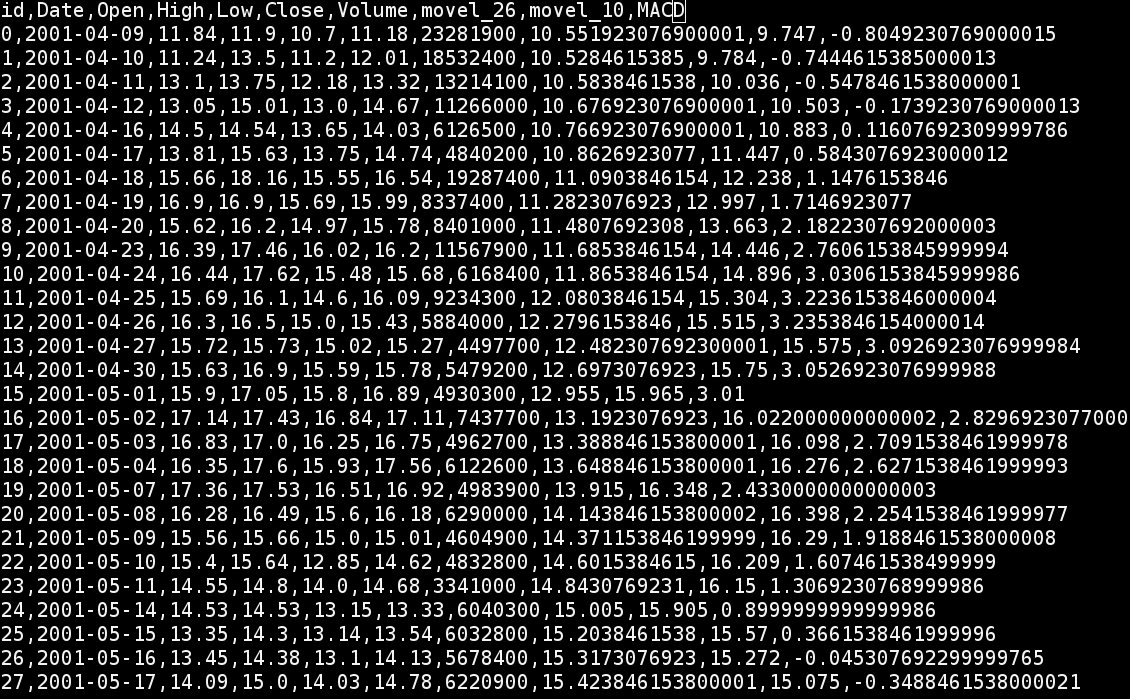
\includegraphics[width=0.8\textwidth, scale=0.5]{dados_formatados}}
	\caption{Exemplo do \textit{DataFrame} com os dados atualizados}
	\fonte{Elaborado pelo autor}
	\label{exec-dados-formatados}
\end{figure}

\section{NORMALIZANDO OS DADOS}
Segundo \citeonline{Luiz}, o evento que antecede a etapa de treinamento de uma RNA é o processo de normalização dos dados de entrada e saída. Como o modelo proposto trabalha com a função de ativação sigmóide, detalhada na Seção 3.3.2, os dados devem ser normalizados entre um intervalo de [0,1]. A normalização consiste em adaptar uma base de dados com valores disintos, o que se aplica à realidade do presente trabalho, onde os valores das ações contam com intervalos de grande oscilação.

Considerando estas informações, duas equações foram especificadas para realizar a normalização e a desnormalização dos dados, com o objetivo de treinar a rede de forma mais eficaz, sendo elas:
\begin{equation}\label{eq:eq-normalizacao}
L_n = (L_o - L_{min}) / (L_{max} - L_{min})
\end{equation}
e
\begin{equation}\label{eq:eq-desnormalizacao}
L_o =  L_n * L_{max} + (1 - L_n) * L_{min},
\end{equation}
onde $L_o$ é o valor à ser normalizado, $L_n$ é o valor normalizado, $L_{min}$ e $L_{max}$ são os valores mínimos e máximos, respectivamente, dentre os valores da variável calculada.

A partir da equação (5.2), foi implementada uma função que normaliza uma determinada coluna de um \textit{DataFrame}. O Código 7 detalha o desenvolvimento do método.
\lstinputlisting[language=Python, label=cod-normalizador, caption=Implementação da função de normalização]{src/normalizador.py}

Para efetuar a desnormalização de um determinado valor, levando em consideração a equação (5.3), foi implementada uma função que realiza este procedimento, detalhada no Código 8.
\lstinputlisting[language=Python, label=cod-desnormalizador, caption=Implementação da função de desnormalização de um valor]{src/desnormalizador.py}  

Tendo em vista o desenvolvimento dos \textit{scripts} demonstrados, Código 7 e Código 8, foi utilizada a biblioteca matplotlib para gerar um gráfico e representar, com clareza, como ficaram os conjuntos de dados após o processo de normalização. O Código 9 detalha este procedimento.

\lstinputlisting[language=Python, label=cod-normalizado-grafico, caption=Classe que gera o gráfico dos dados normalizados]{src/normalizadorGrafico.py}

Após a execução do Código 9, foi renderizado o Gráfico 7 que demonstra os valores de cada empresa distribuidos entre o intervalo [0,1].

\begin{grafico}[h]
	\centering
	\centerline{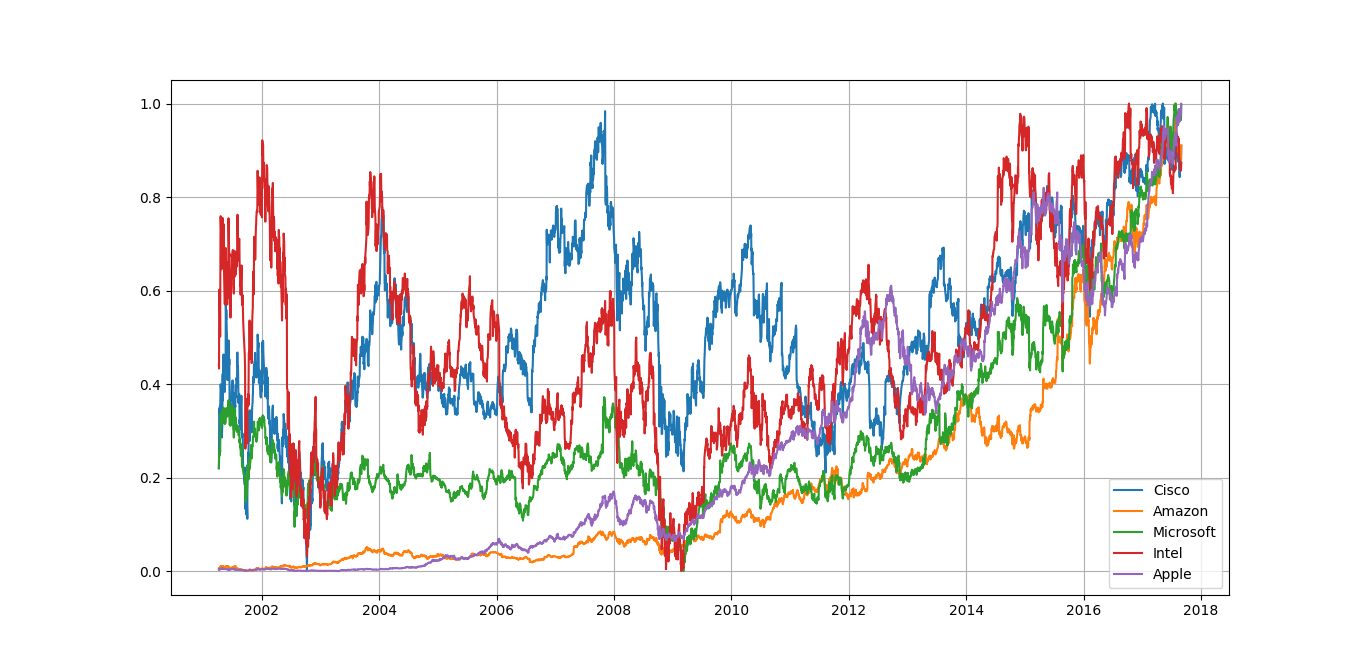
\includegraphics[scale=4]{empresas_normalizado}}
	\caption{Dados normalizados para treinamento}
	\fonte{Elaborado pelo autor}
	\label{exec-intel-coleta}
\end{grafico}